\documentclass[11pt]{article}
\usepackage{url}
\usepackage{hyperref}
\usepackage{latexsym}
\usepackage{multirow}
\usepackage{graphicx}
\graphicspath{}
\usepackage{booktabs}
\usepackage{natbib}
%\bibliographystyle{abbrvnat}
\setcitestyle{authoryear,open={(},close={)}}
\usepackage{float}
\usepackage{listings}


\title{Showcasing the Early Publication World: \linebreak Italy Archives (1501-1600) at Ku Leuven}

\author{Ching-Han Kuo (r0911555) \\ \\
Introduction to Digital Humanities: Final Report \\ {\tt ching-han.kuo@student.kuleuven.be}}

\date{09.01.2023}


\begin{document}
\maketitle

\section{Introduction}
\label{Introduction}
By using metadata from Italy archives (1500-1600) at KU Leuven, this report tries to recreate the publication world during that period. To achieve this goal, first, descriptive statistics are applied to know the data set better. Then, advanced analyses such as linear regression and network analysis are computed to investigate interesting phenomena that may reflect the real world in the past. Finally, the report reveals the adjustments of the original data set to compute the required analysis.

\section{Descriptive Statistics}
\label{label:DescriptiveStatistics}
This section provides an overview of the data set used for this project. The calculation and graphs of this section were generated by Tableau, and the result is displayed on this \href{https://public.tableau.com/app/profile/dhching/viz/DH_Assignment2/ArchivesatKULeuvenItaly1501-1600}{\underline{dashboard}}. The dashboard is an interactive one, meaning that for example, if you would like to find out the specific archives that were published in Venice, just click the location on the map and the whole dashboard will adjust according to it.
\\

\noindent
The top two languages used by archives in this data set are Latin (822, 70.8\%) and Italian (226, 19.77\%), which may indicate that during this period in Italy, Latin is more preferable in the publication than other languages.
\begin{figure}[H]
\centering
\includegraphics[scale=1]{Language table.png}
\includegraphics[scale=0.5]{Language graph.png}
\caption{Table and Graph of Language Distribution}
\label{fig:plutchik}
\end{figure}
\noindent
The distribution of the location where each archive were published is computed and put on a heat map. It displays that Venice can be the centre of publication during the period in Italy because most of the archives (826, 71.15\%) were published there. Other than Venice, Rome (226, 19.47\%) and Florence (83, 7.15\%) may also be important locations for publication.
\begin{figure}[H]
\centering
\includegraphics[scale=1]{Location table.png}
\includegraphics[scale=0.3]{Location graph.png}
\caption{Top Five Table of Location of Publication and Heat Map}
\label{fig:plutchik}
\end{figure}
\noindent
And the majority of these archives (953, 82.08\%) were published after 1540.
\begin{figure}[H]
\centering
\includegraphics[scale=0.8]{Year graph.png}
\caption{Line Graph of Period of Publication}
\label{fig:plutchik}
\end{figure}
\noindent
The distinct count of contributors is 1,559. However, not every person on the name list is the author. Field “700 \$4", which tags the character of each person, need to be applied as a filter that only a person with the tag “aut” in the field will be calculated. The calculation result shows that there are 784 authors in this data set. The average number of archives written by each author is 1.59, and Thomas Aquinas wrote the most archives (16) in this data set.
\begin{figure}[H]
\centering
\includegraphics[scale=1]{Author table.png}
\caption{Total Mean and Top Five Table of Authors}
\label{fig:plutchik}
\end{figure}
\noindent
Finally, The field of “700 \$c” stores some of the titles of people who contributed to the archives. It can be interesting to know what kind of notables were related to the archives, therefore, this field is organised further to analyse. For example, if the title is “Bishop of Nocera” we will extract “Bishop”, or for the title “King of France” we will extract “King”. The result shows that the top three types of notables related to these archives are Cardinal (200, 17.23\%), Pope (194, 16.71\%) and Bishop (88, 7.58\%). This may demonstrate that during this period in Italy, publications were led by the catholic clergies, which can show the impact of religion on the publishing industry in the 16th century in Europe
\begin{figure}[H]
\centering
\includegraphics[scale=1]{Notable table.png}
\includegraphics[scale=0.2]{Notable graph.png}
\caption{Top Five Table and Word Cloud of Notables}
\label{fig:plutchik}
\end{figure}
\section{Statistical Analysis}
In this section, two statistical methods are applied to the data set. Tableau is still the tool to analyse and visualise and the results are also displayed on the dashboards respectively: \href{https://public.tableau.com/app/profile/dhching/viz/TitleXLanguage/NotablesXLanguage}{\underline{hypothesis testing}} and \href{https://public.tableau.com/app/profile/dhching/viz/YearXLocationofPublication/YearXLocationofPublication}{\underline{linear regression}}.
\subsection{Hypothesis Testing: Notables and Language}
Did clergies and non-clergies have different preferences for language usage? The result shows that the proportion of Latin archives connected to Clergy (47.36\%) is significantly higher (p = 0.0167, 95\% CI, two-sided) than the proportion of Latin archives connected to Non-Clergy (35.09\%). Also, the proportion of Non-Latin archives connected to Non-Clergy (23.68\%) is significantly higher (p = 0.0014, 95\% CI, two-sided) than the proportion of Non-Latin archives connected to Clergy (10.08\%). This can demonstrate that for publications during the period in Italy, not only clergies preferred Latin more than non-clergies but also non-clergies preferred Non-Latin more than clergies.
\begin{figure}[H]
\centering
\includegraphics[scale=0.35]{Notable X Language.png}
\caption{Cross Table of Notables and Language}
\label{fig:plutchik}
\end{figure}
\noindent
(The result of the test is computed by the website \href{https://abtestguide.com/calc/}{\underline{ABTestGuide}}, not by Tableau)
\subsection{Linear Regression: Year and Location of Publication}
Did the location of publication change over time? The result shows that the growing trend of the number of publications in non-Venice is stronger than in Venice. Furthermore, if looking only at Rome and Florence, it shows Rome had a very strong growth trend (p lower than 0.0001), but Florence did not. This may indicate that although Venice was still the publishing centre of Italy in this era, Rome was growing rapidly, and according to this trend, it may replace Venice in the future.
\begin{figure}[H]
\centering
\includegraphics[scale=0.35]{Venice X Non-Venice.png}
\includegraphics[scale=0.35]{Rome X Florence.png}
\caption{Scatter Plot of Year and Location of Publication}
\label{fig:plutchik}
\end{figure}

\section{Social Network Analysis}
\label{SocialNetworkAnalysis}
This analysis looks at the contributors working on the archive. The edge list is created by Python, and analysed by Gephi. It can be realised that during the period in Italy, the core of Catholic power was almost the centre of the publishing industry. In addition, it seems that the hierarchical system at that time was also reflected in the publishing industry. People with titles and those without titles almost belong to different network clusters.
\begin{figure}[H]
\centering
\includegraphics[scale=0.5]{Network table.png}
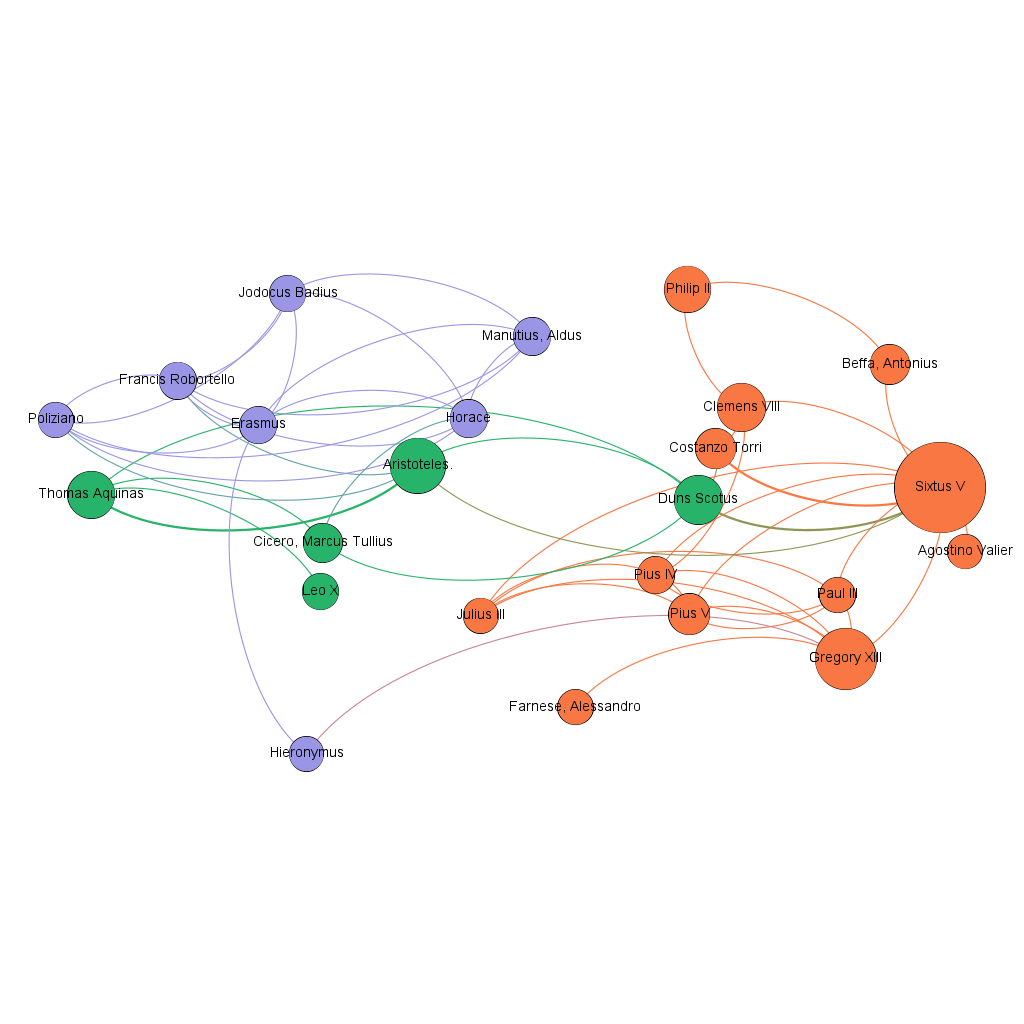
\includegraphics[scale=0.1]{Network.png}
\caption{Top Ten Table and Graph of Social Network Analysis ($Degree Centrality > 20$)}
\label{fig:plutchik}
\end{figure}

\section{Data-set Adjustment}
\label{DataSetAdjustment}
Because the original CSV is imported from OpenRefine, OpenRefine can detect which rows belong to the same archive, but other tools like Tableau can not. Therefore, it is needed to go back to OpenRefine and use the fill-down function on the column that is used as ID (“001” in this case).
\\
Some analysis in the report requires categorising the items in a column. For example, to conduct analytic in 3-1, language (041 \$a) needs to be categorised into Latin and Non-Latin, and the Title of people (700 \$c) needs to be categorised into Clergy and Non-Clergy. It is not necessary to go back to OpenRefine for the categorization because tools like Tableau have similar applications.
\\
Finally, the biggest obstacle to analysing this data set is the inconsistency of data. First, due to the variety of languages of archives, for example, when importing the data set into Python, white space in some strings will be \/xa0, which is because they are coded in Latin-1 instead of UTF-8, and need to be eliminated before analysing. The second is the inconsistency in data entry. For example, the location of publication (“264 \$a”) is often inconsistent, some are cities, some are countries, and some are provinces. And also for the year of publication (“264 \$c”), some are intervals and some are individual years. For these, it is needed to go back to OpenRefine and use the function of text facet to modify them manually.

\section{Conclusion}
\label{Conclusion}
Through the analysis of this data set, this report discovers several noteworthy phenomena that may allow us to understand the world of the publication of Italy in the 16th century. We see, for example, the influence of Catholic Church on publishing, and the difference in language choice by status of a person, and we witness the growth of the publishing industry in Rome. In addition, this report teaches us that when analysing this type of data sets in the future, it is needed to keep in mind that data inconsistencies may encounter and need to reserve time or resource ahead for manual adjustment.

\end{document}